% ==============================================================================
% chapters/ch06_ai_prompt_engineering.tex
% บทที่ 6: วิศวกรรมชุดคำสั่งปัญญาประดิษฐ์และสถาปัตยกรรมแอปพลิเคชัน
% ตามมาตรฐาน rbru-academic-formatter & rbru-latex-textbook-builder
% ==============================================================================

\chapter{วิศวกรรมชุดคำสั่งปัญญาประดิษฐ์และสถาปัตยกรรมแอปพลิเคชัน}
\label{chap:ch06}

\section*{แผนบริหารการสอนประจำบทที่ 6}
\addcontentsline{toc}{section}{แผนบริหารการสอนประจำบทที่ 6}

\noindent\textbf{หัวข้อเนื้อหาประจำบท}
\begin{enumerate}
    \item ปัญหาการสูญเสียโทเค็นและหลักการบีบอัดบริบทระบบ (Token Efficiency System Context)
    \item การออกแบบและสั่งการ AI สร้าง Web Application Dashboard ด้วย Streamlit และ FastAPI
    \item การออกแบบและสั่งการ AI สร้าง Smartphone Application ด้วย Flutter และ Edge AI
    \item การเชื่อมต่อฮาร์ดแวร์เซนเซอร์วัดธาตุอาหารดิน NPK ผ่าน Bluetooth Low Energy (BLE)
    \item มาตรฐานไฟล์คอนฟิกสำหรับสภาพแวดล้อมการพัฒนาสมัยใหม่ (.cursorrules, AGENTS.md, copilot-instructions.md)
    \item สถาปัตยกรรมและระเบียบการจัดทำตำราวิชาการ XeLaTeX ตามมาตรฐาน มรภ.รำไพพรรณี
\end{enumerate}

\noindent\textbf{วัตถุประสงค์เชิงพฤติกรรม}
\begin{enumerate}
    \item เพื่อให้ผู้เรียนสามารถอธิบายโครงสร้างคอนเทกต์แบบกระชับพิเศษ (Ultra-Compact Context) ได้อย่างถูกต้อง
    \item เพื่อให้ผู้เรียนสามารถประยุกต์ใช้ Prompt Engineering สั่งสร้างเว็บแดชบอร์ดและแอปพลิเคชันสมาร์ทโฟนได้อย่างสมบูรณ์
    \item เพื่อให้ผู้เรียนสามารถเชื่อมโยงโมเดล Edge AI (ONNX และ TFLite) เข้ากับส่วนต่อประสานผู้ใช้ได้จริง
    \item เพื่อให้ผู้เรียนสามารถตั้งค่าไฟล์ควบคุมพฤติกรรม AI ใน Cursor, Google Antigravity และ VS Code ได้อย่างถูกต้อง
\end{enumerate}

\noindent\textbf{กิจกรรมการเรียนการสอน}
\begin{enumerate}
    \item บรรยายเชิงปฏิบัติการเรื่อง Token Economy และสถาปัตยกรรม CLEAR Prompting
    \item ฝึกปฏิบัติการสั่งการ AI คู่คิด (Pair Programming) ผ่าน Cursor และ Google Antigravity
    \item ปฏิบัติการทดสอบรันแอปพลิเคชัน Web Dashboard และ Flutter Mobile Edge AI จากชุด Starter Template
    \item อภิปรายกลุ่มย่อยเกี่ยวกับการนำชุดคำสั่งไปประยุกต์ใช้กับโจทย์การเกษตรในพื้นที่จริง
\end{enumerate}

\noindent\textbf{สื่อการเรียนการสอน}
\begin{enumerate}
    \item เอกสารคู่มือปฏิบัติการ Digital Agri xAI บทที่ 6
    \item คลังชุดคำสั่งและเทมเพลต ai\_prompts\_kit และโค้ดตัวอย่างใน GitHub Repository
    \item สภาพแวดล้อมการพัฒนา Google Colab, Cursor Editor และ VS Code
    \item ชุดทดสอบโมเดล ONNX Runtime และ TFLite จำลอง
\end{enumerate}

\noindent\textbf{การประเมินผล}
\begin{enumerate}
    \item ประเมินจากการมีส่วนร่วมและการตอบคำถามในชั้นเรียน
    \item ประเมินจากความถูกต้องของไฟล์คอนฟิกและผลการรันเว็บแดชบอร์ดที่สร้างขึ้น
    \item ประเมินจากการตอบคำถามทบทวนท้ายบทที่ 6 ได้อย่างถูกต้องครบถ้วน
\end{enumerate}

\newpage

% ------------------------------------------------------------------------------
% เนื้อหาบทที่ 6
% ------------------------------------------------------------------------------

\academicsection{บริบทระบบและการบีบอัดคอนเทกต์แบบประหยัดโทเค็น}

ในการพัฒนาซอฟต์แวร์และระบบปัญญาประดิษฐ์ทางการเกษตรยุคปัจจุบัน การใช้งานปัญญาประดิษฐ์ช่วยเขียนโค้ด (AI Coding Assistants) เช่น Cursor, VS Code Copilot และ Google Antigravity มีบทบาทสำคัญอย่างยิ่ง อย่างไรก็ดี ปัญหาหลักที่นักวิจัยและผู้เข้าอบรมมักประสบคือ \textbf{ปัญหาความสูญเปล่าของโทเค็น (Token Waste)} และการที่แบบจำลองภาษาขนาดใหญ่ (LLMs) สูญเสียบริบทของระบบอันเนื่องมาจากการป้อนข้อมูลที่เยิ่นเย้อเกินความจำเป็น

ด้วยเหตุนี้ โครงการ Digital Agri xAI จึงได้พัฒนากรอบสถาปัตยกรรม \textbf{Ultra-Compact Token-Efficient Context} ซึ่งเป็นการบีบอัดข้อมูลสเปกระบบทั้งหมดให้อยู่ในรูปแบบ YAML ขนาดย่อไม่เกิน 350 โทเค็น แต่ครอบคลุมข้อมูลสำคัญครบถ้วนทั้ง 4 มิติ ได้แก่ โดเมนข้อมูล (4 โดเมนหลัก 16 คลาส), รูปแบบโมเดล (ONNX สำหรับเว็บ และ TFLite Quantized สำหรับมือถือ), พารามิเตอร์เซนเซอร์ตรวจวัดดิน (NPK, pH, ความชื้น, อุณหภูมิ), และกฎเกณฑ์ทางวิศวกรรมซอฟต์แวร์ (Clean Architecture, Zero Overflow, และโทนสี Dark Glassmorphism)

\begin{academicNote}
\textbf{หลักการ CLEAR Prompting Framework สำหรับเกษตรดิจิทัล}\par
การเขียนคำสั่งให้มีประสิทธิภาพสูงสุดต้องประกอบด้วย:
\textbf{C}ontext (บริบทระบบที่ชัดเจน), \textbf{L}imitations (ข้อจำกัดด้านความหน่วงและหน่วยความจำ), \textbf{E}xamples (ตัวอย่างเอาต์พุตที่ต้องการ), \textbf{A}ctions (คำสั่งระบุการกระทำที่ชัดแจ้ง), และ \textbf{R}ules (กฎการเขียนโค้ดที่เคร่งครัด)
\end{academicNote}

\academicsection{การสั่งสร้างเว็บแดชบอร์ดศูนย์สั่งการแปลงเกษตร}

เว็บแอปพลิเคชันศูนย์สั่งการ (Central Field Dashboard) ทำหน้าที่เป็นจุดรวมข้อมูลโทรมาตร (Telemetry) และการวินิจฉัยภาพถ่ายจากแปลงเกษตร โดยใช้เทคโนโลยี Streamlit สำหรับการแสดงผลแบบโต้ตอบเร็ว และ FastAPI สำหรับการให้บริการโมเดลความเร็วสูงผ่านเครือข่าย

โครงสร้างคำสั่งสั่งสร้างแดชบอร์ดได้รับการออกแบบให้ระบุฟังก์ชันสำคัญ 4 แท็บ ได้แก่:
\begin{enumerate}
    \item \textbf{Real-time Telemetry HUD:} แสดงเกจวัดธาตุอาหาร N-P-K (มิลลิกรัมต่อกิโลกรัม), ความเป็นกรด-ด่างของดิน (pH), ความชื้น และอุณหภูมิ พร้อมไฟสถานะ Online Beacon สีเขียวกระพริบ
    \item \textbf{AI Visual Diagnosis:} ระบบลากวางภาพถ่ายดินหรือใบพืช ส่งเข้าสู่โมเดล MobileNetV3 แบบ In-Process ผ่าน ONNX Runtime เพื่อวินิจฉัยโรคและธาตุอาหารโดยมีค่าความหน่วงต่ำกว่า 20 มิลลิวินาที
    \item \textbf{Crop Recommender:} ระบบคำนวณพืชที่เหมาะสม 3 อันดับแรกตามค่า N-P-K และ pH ด้วยอัลกอริทึม Nearest Centroid พร้อมคำนวณสูตรปุ๋ยสั่งตัดรายแปลง
    \item \textbf{Data Export:} การส่งออกรายงานผลการวินิจฉัยในรูปแบบ JSON สำหรับระบบภายนอก และ Markdown Card สำหรับสรุปผลให้เกษตรกร
\end{enumerate}

\academicsection{การสั่งสร้างสมาร์ทโฟนแอปพลิเคชัน Edge AI ด้วย Flutter}

สำหรับเกษตรกรในพื้นที่ห่างไกลซึ่งการเชื่อมต่อสัญญาณอินเทอร์เน็ตอาจไม่เสถียร สถาปัตยกรรมแอปพลิเคชันสมาร์ทโฟนต้องทำงานในรูปแบบ \textbf{Offline-First Edge AI} 100\% โดยใช้เฟรมเวิร์ก Flutter เวอร์ชัน 3.x ร่วมกับภาษา Dart

การสั่งการ AI ให้สร้างโมบายล์แอปพลิเคชันที่มีคุณภาพสูง ปฏิบัติตามโครงสร้าง Clean Architecture (MVVM ร่วมกับ Provider State Management) โดยแบ่งเลเยอร์ซอฟต์แวร์เป็น 3 ส่วนหลัก ได้แก่:
\begin{enumerate}
    \item \textbf{Data Layer:} โครงสร้างข้อมูล \texttt{DiagnosticResult} และ \texttt{SoilSensorData} พร้อมการจัดเก็บแคชข้อมูลออฟไลน์และพิกัดภูมิศาสตร์ (GPS Geotagging) ลงฐานข้อมูล SQLite ภายในเครื่อง
    \item \textbf{Domain \& Logic Layer:} การอนุมานโมเดลผ่าน \texttt{ScannerProvider} ซึ่งเชื่อมโยงไลบรารี \texttt{tflite\_flutter} ประมวลผลภาพขนาด $224 \times 224$ พิกเซล บนชิปเร่งความเร็ว NPU/GPU ภายในอุปกรณ์โดยตรง
    \item \textbf{Presentation Layer:} ออกแบบหน้าจอตามมาตรฐาน Responsive ไร้ปัญหา RenderFlex Overflow คุมโทนสี Dark Obsidian (\#090D16) เส้นขอบนีออนมรกต (\#10B981) และกรอบเล็งเป้าหมาย (Target Reticle) พร้อมการ์ดลอยแก้ว (Floating Glassmorphic Card)
\end{enumerate}

ดังแสดงในภาพที่ \ref{fig:mobile_camera_scanner} หน้าจอแอปพลิเคชันส่องกล้องวินิจฉัยสุขภาพพืชและตรวจจับโรคใบจุดออฟไลน์ สามารถระบุคลาสการวินิจฉัย เช่น แอนแทรคโนส (Anthracnose) หรือการขาดธาตุอาหาร แสดงค่าความมั่นใจของโมเดล (Confidence Score) สูงถึง 96.8\% พร้อมปุ่มบันทึกประวัติการสำรวจแปลงแบบออฟไลน์

\begin{figure}[htbp]
\centering
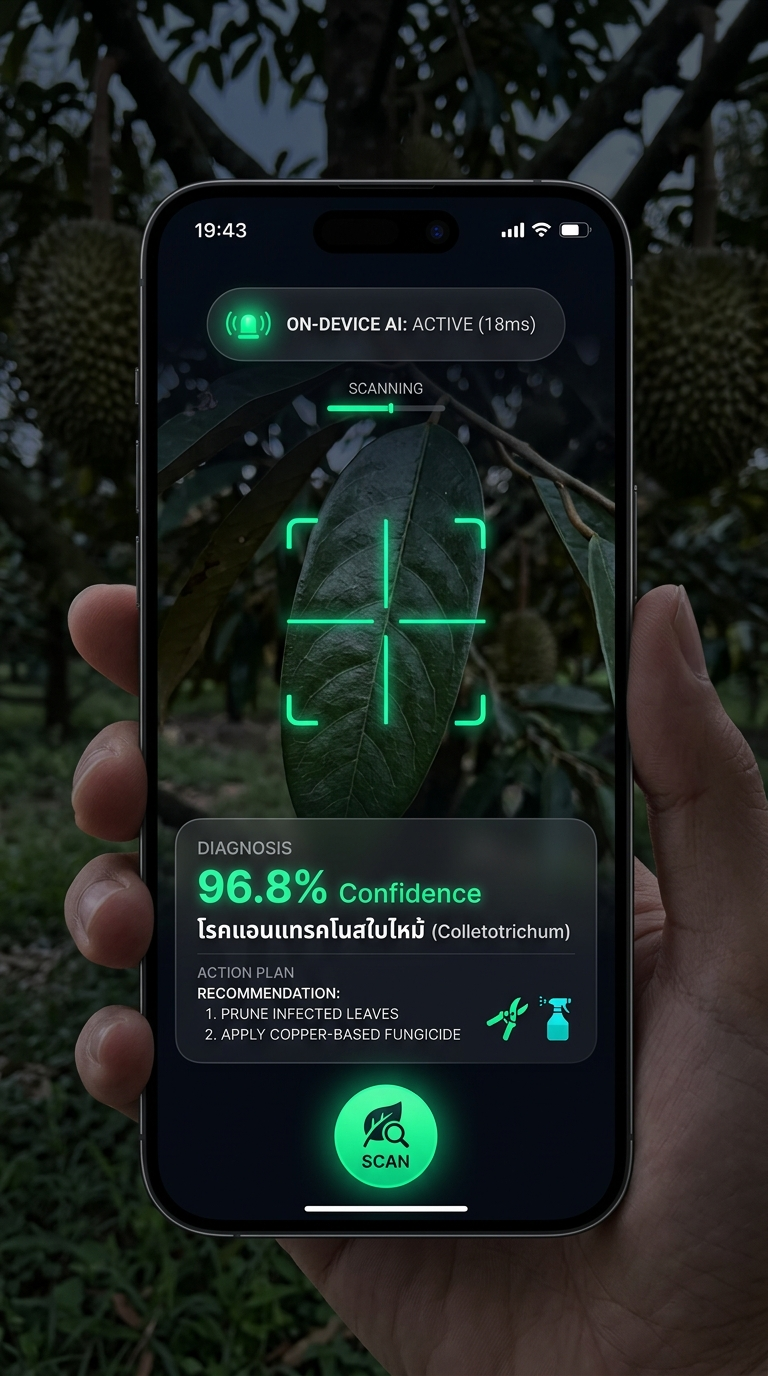
\includegraphics[width=0.52\textwidth]{figures/mobile_screen_camera_scanner.jpg}
\caption{หน้าจอแอปพลิเคชันสมาร์ทโฟนส่องกล้อง Edge AI วินิจฉัยสุขภาพพืชและโรคใบจุดออฟไลน์แบบเรียลไทม์}
\label{fig:mobile_camera_scanner}
\end{figure}

\academicsection{การเชื่อมต่อฮาร์ดแวร์เซนเซอร์ดิน NPK ผ่าน Bluetooth Low Energy}

นอกจากการประมวลผลสัญญาณภาพแล้ว ข้อมูลทางเคมีและกายภาพของดินจากหัวโพรบ RS485 Modbus ที่แปลงสัญญาณผ่านโมดูลบลูทูธพลังงานต่ำ (ESP32 BLE) ถือเป็นหัวใจสำคัญอย่างยิ่งของการวิเคราะห์ความสมบูรณ์ของดินรายแปลง

ชุดคำสั่งสำหรับสั่ง AI สร้างหน้าจอเชื่อมต่อเซนเซอร์ดิน กำหนดให้ใช้ไลบรารี \texttt{flutter\_blue\_plus} พร้อมระบบค้นหาและจับคู่อุปกรณ์รอบตัว (Device Scanning) การอ่านค่า Characteristic ของเซนเซอร์ และการแปลงค่าไบต์ดิบ (Raw Hex Bytes) เป็นค่าทางกายภาพจริง

ดังแสดงในภาพที่ \ref{fig:mobile_ble_sensor} หน้าจอแสดงผลโทรมาตรเซนเซอร์ดิน (Soil Telemetry \& Sensor HUD) ประกอบด้วยเกจวัดวงกลมไฮเทคและมาตรวัดค่าเคมีดิน 6 พารามิเตอร์หลัก ได้แก่ ไนโตรเจน (N), ฟอสฟอรัส (P), โพแทสเซียม (K), ความเป็นกรด-ด่าง (pH: 5.8), ความชื้น (Moisture: 72\%) และอุณหภูมิดิน (28.4$^\circ$C) พร้อมการ์ดสรุปคำแนะนำการปรับสภาพดินและสูตรปุ๋ยสั่งตัดที่คำนวณโดยระบบผู้เชี่ยวชาญแบบอัตโนมัติ

\begin{figure}[htbp]
\centering
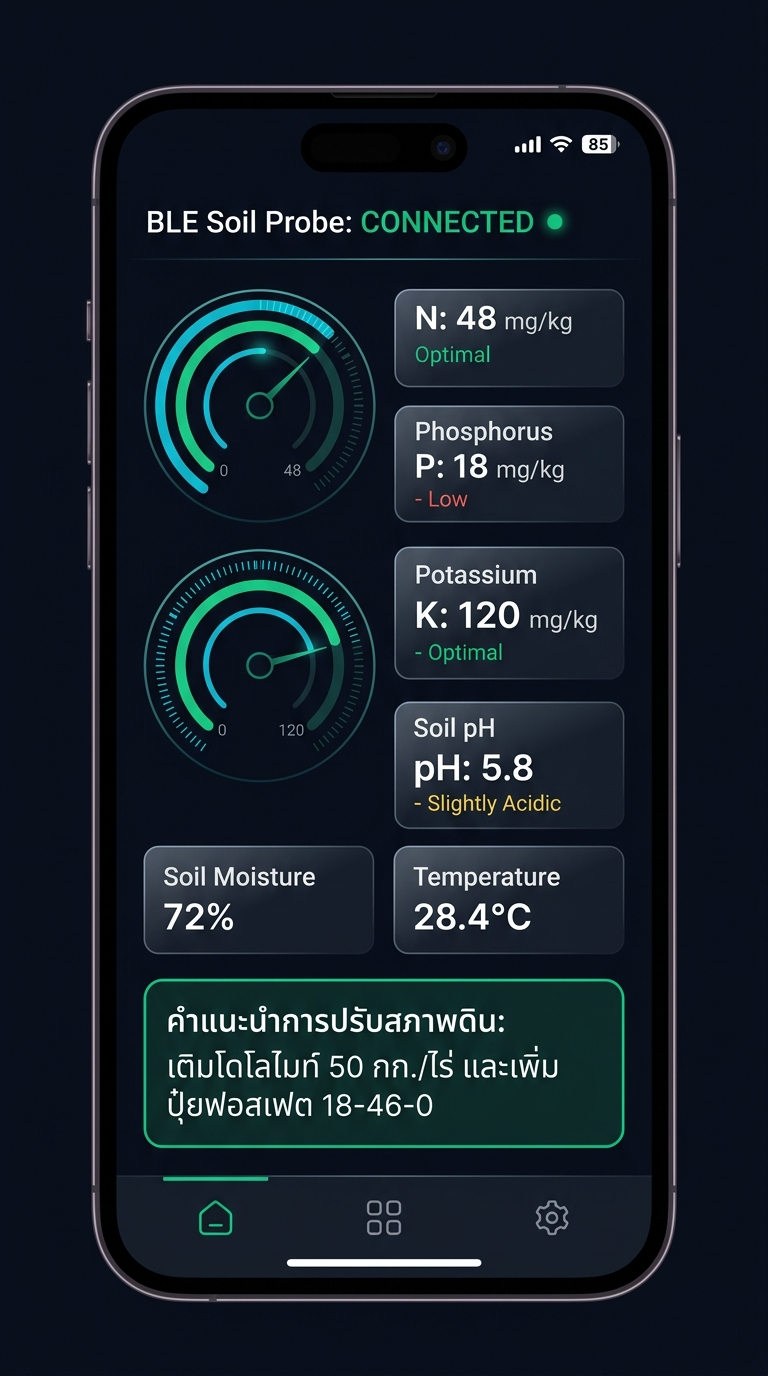
\includegraphics[width=0.52\textwidth]{figures/mobile_screen_ble_sensor.jpg}
\caption{หน้าจอแสดงผลข้อมูลโทรมาตรเซนเซอร์ดิน NPK และ pH ผ่านบลูทูธพลังงานต่ำ (BLE) พร้อมคำแนะนำปุ๋ยสั่งตัด}
\label{fig:mobile_ble_sensor}
\end{figure}

\academicsection{มาตรฐานไฟล์คอนฟิกสำหรับสภาพแวดล้อมการพัฒนาสมัยใหม่}

เพื่อให้ AI Coding Assistants ปฏิบัติตามกฎเกณฑ์ทางวิศวกรรมซอฟต์แวร์และข้อกำหนดทางเกษตรวิทยาอย่างเคร่งครัด ได้มีการจัดทำไฟล์คอนฟิกมาตรฐานไว้ 3 รูปแบบ:

\begin{enumerate}
    \item \textbf{\texttt{.cursorrules}:} สำหรับใช้งานใน Cursor AI Editor ระบุการจำแนกประเภทข้อมูล กฎการเขียนโค้ดภาษา Python/Dart และโทนสี Dark Obsidian (\#090D16) ผสานสีเขียวมรกต (\#10B981)
    \item \textbf{\texttt{AGENTS.md}:} สำหรับใช้งานใน Google Antigravity และ Agentic Pair Programming IDE กำหนดเป้าหมายระบบ กฎการคอมไพล์ทดสอบ และการรักษามาตรฐานวิชาการ
    \item \textbf{\texttt{copilot-instructions.md}:} สำหรับใช้งานใน VS Code ร่วมกับ GitHub Copilot กำหนดมาตรฐานโค้ด ข้อห้ามเรื่อง Placeholder stubs และการใช้คำศัพท์ภาษาไทยที่ถูกต้อง
\end{enumerate}

\begin{table}[htbp]
\centering
\caption{การเปรียบเทียบคุณสมบัติและสภาพแวดล้อมของชุดคำสั่ง AI Prompts Kit}
\label{tab:prompt_kit_comparison}
\fontsize{8.5}{11}\selectfont
\begin{tabularx}{\textwidth}{p{2.1cm}Xp{1.9cm}r}
\toprule
\textbf{ชุดคำสั่ง} & \textbf{เป้าหมายการประยุกต์ใช้} & \textbf{เทคโนโลยี} & \textbf{โทเค็น} \\
\midrule
System Context & กำหนดบริบททั้งระบบในภาพรวม & YAML Spec & $\sim$320 \\
Web Dashboard & ศูนย์สั่งการและแสดงผลโทรมาตรแปลง & Streamlit/FastAPI & $\sim$480 \\
Mobile Edge AI & แอปพลิเคชันกล้องวินิจฉัยดินและโรคพืช & Flutter/TFLite & $\sim$520 \\
BLE Sensors & เชื่อมต่อหัวโพรบวัด NPK และ pH ดิน & Flutter/BLE & $\sim$450 \\
IDE Configs & ควบคุมพฤติกรรม AI ในระดับโปรเจกต์ & Cursor/AGENTS & $\sim$350 \\
LaTeX Book & จัดทำรูปเล่มตำราและคู่มือวิชาการ 6x9 & XeLaTeX/TikZ & $\sim$650 \\
\bottomrule
\end{tabularx}
\end{table}

\academicsection{สถาปัตยกรรมและระเบียบการจัดทำตำราวิชาการ XeLaTeX}

การเผยแพร่องค์ความรู้จากการวิจัยจำเป็นต้องจัดทำเป็นเอกสารตำราวิชาการที่มีคุณภาพสูงและถูกต้องตามระเบียบของมหาวิทยาลัยราชภัฏรำไพพรรณี (อ้างอิงมาตรฐาน \texttt{rbru-academic-formatter} และ \texttt{thai-academic-latex-formatting}) โดยมีข้อกำหนดหลักดังนี้:

\begin{enumerate}
    \item \textbf{ขนาดรูปเล่มและฟอนต์:} ขนาดรูปเล่ม 6 $\times$ 9 นิ้ว (Royal Octavo) เว้นขอบใน 1.0 นิ้วสำหรับเข้าเล่ม ฟอนต์หลัก TH Sarabun New / Sarabun ระยะบรรทัด 1.18 เท่า พร้อมระบบตัดคำภาษาไทย \texttt{\textbackslash XeTeXlinebreaklocale "th"}
    \item \textbf{ย่อหน้าและหัวข้อ:} ย่อหน้าแรก 3em ไม่เว้นวรรคระหว่างย่อหน้า บังคับย่อหน้าแรกหลังหัวข้อด้วย \texttt{indentfirst} เริ่มต้นบทใหม่ที่หน้าคี่เสมอ พร้อมใช้ \texttt{\textbackslash needspace} ป้องกันหัวข้อตกค้างท้ายหน้า
    \item \textbf{คำบรรยายภาพและตาราง:} ใช้ป้าย "ภาพที่" และ "ตารางที่" คั่นด้วยเว้นวรรค 1 เคาะ ห้ามมีเครื่องหมายทวิภาค (:) โดยคำบรรยายตารางทั้งหมดต้องจัดชิดซ้ายทั้งเล่ม
    \item \textbf{สถาปัตยกรรมปกคู่:} ปกนอกภาพประกอบ 3D Pixar สัดส่วน 2:3 แบบ Full-bleed TikZ ซ้อนเงาตัวอักษรโปร่งใส ไร้กล่องทึบบดบังภาพ พร้อมปกในระบุข้อมูลวิชาการครบถ้วน
\end{enumerate}

\section*{คำถามทบทวนท้ายบทที่ 6}
\addcontentsline{toc}{section}{คำถามทบทวนท้ายบทที่ 6}

\begin{enumerate}
    \item จงอธิบายสาเหตุและผลกระทบของปัญหาการสูญเสียโทเค็น (Token Waste) ในการสั่งการ AI พร้อมอธิบายแนวทางการแก้ไขด้วย Ultra-Compact Context
    \item จงเปรียบเทียบความแตกต่างระหว่างการประมวลผลแบบ Cloud AI และ In-Process Edge AI ในระบบตรวจวิเคราะห์ดินทางการเกษตร ทั้งในด้านความหน่วงและความเป็นส่วนตัวของข้อมูล
    \item เพราะเหตุใดการพัฒนาแอปพลิเคชันสมาร์ทโฟนสำหรับเกษตรกรจึงต้องใช้แนวคิด Offline-First และโมเดล Quantized TFLite มีข้อดีอย่างไร
    \item จงอธิบายขั้นตอนการเชื่อมต่อหัวโพรบวัด NPK ในดินผ่าน Bluetooth Low Energy (BLE) และการประมวลผลค่าเพื่อคำนวณสูตรปุ๋ยสั่งตัด
    \item จงระบุความสำคัญของการกำหนดไฟล์ \texttt{.cursorrules} และ \texttt{AGENTS.md} ต่อการควบคุมคุณภาพซอฟต์แวร์ในการเขียนโค้ดร่วมกับ AI
    \item จงอธิบายข้อกำหนดสำคัญในการจัดทำเอกสารตำราวิชาการ XeLaTeX ตามมาตรฐานของ มรภ.รำไพพรรณี ทั้งในด้านการจัดหน้า คำบรรยายภาพ/ตาราง และสถาปัตยกรรมปกคู่
\end{enumerate}

\clearpage
